\documentclass{elektr}
\usepackage{hyperref}
\hypersetup{colorlinks=true,urlcolor=black,citecolor=blue}
\usepackage{amsfonts,amssymb,amsmath,amsgen,amsopn,amsbsy,theorem,graphicx}
\usepackage[utf8]{inputenc}
\usepackage[english]{babel}
\usepackage{multirow,array}
\usepackage[dvipsnames]{xcolor}
\usepackage[pagewise]{lineno}
\linenumbers
\usepackage{float}
\raggedbottom
\usepackage{enumitem}
\setlist{noitemsep, topsep=1pt}
\setlength{\textfloatsep}{6pt plus 1pt minus 2pt}
\setlength{\floatsep}{5pt plus 1pt minus 2pt}
\setlength{\intextsep}{6pt plus 1pt minus 2pt}
\setlength{\abovecaptionskip}{3pt}
\setlength{\belowcaptionskip}{2pt}
\renewcommand{\arraystretch}{0.94}

\yil{}
\vol{}
\fpage{}
\lpage{}
\doi{}

\title{QLoRA Fine-Tuning for Consumer Complaint Classification}

\author[TAN and BAKIR]{
\textbf{Muhammet TAN$^{1,}$\thanks{muhammet.tan@sivas.edu.tr}~, Halit BAKIR$^{1}$}\\
$^{1}$Department of Computer Engineering, Sivas University of Science and Technology, Sivas, Turkey\\
Muhammet TAN: \url{https://orcid.org/0009-0004-9430-372X}\\
Halit BAKIR: \url{https://orcid.org/0000-0003-3327-2822}\\[1.8em]
\rec{}
\acc{}
\finv{}
}

\def\E{\ifmmode{\mathbb E}\else{$\mathbb E$}\fi} %natural numbers
\def\N{\ifmmode{\mathbb N}\else{$\mathbb N$}\fi} %natural numbers
\def\R{\ifmmode{\mathbb R}\else{$\mathbb R$}\fi} %real numbers
\def\Q{\ifmmode{\mathbb Q}\else{$\mathbb Q$}\fi} %rational numbers
\def\C{\ifmmode{\mathbb C}\else{$\mathbb C$}\fi} %complex numbers
\def\H{\ifmmode{\mathbb H}\else{$\mathbb H$}\fi} %complex numbers
\def\Z{\ifmmode{\mathbb Z}\else{$\mathbb Z$}\fi} %integers
\def\P{\ifmmode{\mathbb P}\else{$\mathbb P$}\fi} %real numbers
\def\T{\ifmmode{\mathbb T}\else{$\mathbb T$}\fi} %real numbers
\def\SS{\ifmmode{\mathbb S}\else{$\mathbb S$}\fi} %real numbers
\def\DD{\ifmmode{\mathbb D}\else{$\mathbb D$}\fi} %real numbers

\renewcommand{\a}{\alpha}
\renewcommand{\b}{\beta}
\renewcommand{\d}{\delta}
\newcommand{\D}{\Delta}
\newcommand{\e}{\epsilon}
\newcommand{\var}{\varepsilon}
\newcommand{\g}{\gamma}
\newcommand{\la}{\lambda}
\newcommand{\La}{\Lambda}
\newcommand{\lan}{\langle}
\newcommand{\ran}{\rangle}
\newcommand{\n}{\nabla}
\newcommand{\va}{\varphi}
\newcommand{\s}{\sigma}
\newcommand{\Sig}{\Sigma}
\renewcommand{\t}{\tau}
\renewcommand{\th}{\theta}
\newcommand{\Om}{\Omega}
\newcommand{\om}{\omega}
\newcommand{\pa}{\partial}
\newcommand{\up}{\upsilon}
\newcommand{\vp}{\varphi}
\newcommand{\z}{\zeta}





\newcommand{\bse}{\begin{subequations}}
\newcommand{\ese}{\end{subequations}}
\newcommand{\ben}{\begin{enumerate}}
\newcommand{\een}{\end{enumerate}}
\newcommand{\bens}{\begin{enumerate*}}
\newcommand{\eens}{\end{enumerate*}}
\newcommand{\be}{\begin{equation}}
\newcommand{\ee}{\end{equation}}
\newcommand{\bea}{\begin{eqnarray}}
\newcommand{\eea}{\end{eqnarray}}
\newcommand{\baa}{\begin{eqnarray*}}
\newcommand{\eaa}{\end{eqnarray*}}
\newcommand{\bc}{\begin{center}}
\newcommand{\ec}{\end{center}}
\newcommand{\ol}{\overline}
\newcommand{\ul}{\underline}
\newcommand{\ov}{\overbrace}
\newcommand{\uv}{\underbrace}
\newcommand{\Ra}{\Rightarrow}
\newcommand{\ra}{\rightarrow}
\newcommand{\ds}{\displaystyle}
\newcommand{\vs}{\vspace}


\newcommand{\IR}{\mbox{I \hspace{-0.2cm}R}}
\newcommand{\IN}{\mbox{I \hspace{-0.2cm}N}}



%% \theoremstyle{plain} %% This is the default

\newtheorem{theorem}{Theorem}%[section]

\theoremstyle{corollary}
\newtheorem{corollary}{Corollary}

\theoremstyle{lemma}
\newtheorem{lemma}{Lemma}

\theoremstyle{proposition}
\newtheorem{proposition}{Proposition}

\theoremstyle{axiom}
\newtheorem{axiom}{Axiom}

\theoremstyle{conjecture}
\newtheorem{conjecture}{Conjecture}

\theoremstyle{example}
\newtheorem{example}{Example}

\theoremstyle{definition}
\newtheorem{definition}{Definition}%[section]

\theoremstyle{remark}
\newtheorem{remark}{Remark}%[section]
\newtheorem{notation}{Notation}


\newtheorem{question}{Question}%[section]
\newtheorem{construction}{Construction}

\newtheorem{athm}{Theorem}
\renewcommand{\theathm}{\Alph{athm}}



\setcounter{page}{1}

\begin{document}
\maketitle

\begin{abstract}
Consumer financial complaint classification is a practically important text classification task for regulatory triage, customer-service routing, and institutional risk monitoring. Although locally served open-weight large language models can be used as zero-shot complaint classifiers, it remains necessary to determine whether the same models can be substantially improved through task-specific adaptation without sacrificing reproducibility or data isolation. This study evaluates that transition using a leakage-controlled parameter-efficient fine-tuning protocol. Legacy zero-shot subsets created before fine-tuning are excluded from training and preserved as a paired benchmark; the remaining corpus is split into train, validation, and internal test partitions with duplicate-aware safeguards. Qwen3-8B and Llama 3.1-8B are fine-tuned using QLoRA under a fixed two-epoch protocol and evaluated across three random seeds. On the internal test set, Qwen3-8B improves from 0.6294 to 0.8350 macro-F1, while Llama 3.1-8B improves from 0.6189 to 0.8378. On the legacy benchmark, mean macro-F1 improves by 0.1853 and 0.2289, respectively. Wilcoxon signed-rank tests over the 12 legacy subsets show consistent paired gains for accuracy, macro-F1, and weighted F1. The largest class-level improvements occur for debt collection, a difficult category frequently confused with credit reporting in zero-shot inference. These results indicate that QLoRA fine-tuning provides a robust, reproducible, and locally deployable improvement over zero-shot open-source LLM classification for consumer complaint triage.
\keywords{Consumer complaint classification, large language models, QLoRA, parameter-efficient fine-tuning, zero-shot learning, data leakage, CFPB}
\end{abstract}

\section{Introduction}

The Consumer Financial Protection Bureau (CFPB) complaint database is a large public corpus of consumer narratives describing financial disputes, product failures, debt collection issues, credit reporting problems, and banking complaints. Accurate classification of such narratives is important for regulatory monitoring, institutional triage, and the prioritisation of consumer-service workflows. The task is challenging because complaint narratives often mention multiple financial products, contain noisy informal descriptions, and must nevertheless be mapped to a single constrained product category.

Recent work has explored large language models (LLMs) for zero-shot complaint classification. In zero-shot settings, models receive the candidate categories in the prompt and must return a valid label without task-specific training. This is attractive for complaint triage because new product taxonomies or institutional routing schemes may be introduced before large labelled datasets are available. However, zero-shot classification also raises practical issues: models can confuse overlapping financial products, output labels outside the allowed taxonomy, and show sensitivity to prompt and deployment details. Once a local zero-shot baseline is established for a given open-weight model, the next methodological question is how much performance can be gained through parameter-efficient fine-tuning under a fair and leakage-controlled protocol.

This paper addresses that question. The central novelty is not a new model architecture or a new fine-tuning algorithm. Instead, the contribution is a reproducible applied evaluation and leakage-safe benchmark extension of a zero-shot experimental setting. We introduce a duplicate-aware train/validation/test split, exclude all legacy zero-shot subsets from model selection and training, and evaluate paired zero-shot versus QLoRA fine-tuned models in the same Hugging Face pipeline. Unlike single-model or single-seed complaint-classification studies, the present work evaluates the zero-shot-to-fine-tuned transition under paired, multi-seed, multi-model, leakage-controlled conditions. Two different 8B-class open-source model families, Qwen3-8B and Llama 3.1-8B, are evaluated across three random seeds. The final evaluation uses both a held-out internal test set and preserved legacy zero-shot subsets.

The contributions are as follows:
\begin{enumerate}
    \item We provide a leakage-controlled transition from zero-shot open-source LLM inference to QLoRA fine-tuning for CFPB consumer complaint classification.
    \item We preserve pre-existing zero-shot subsets as a legacy benchmark and explicitly exclude them from fine-tuning and model selection.
    \item We compare base zero-shot and fine-tuned models within the same Hugging Face quantised inference pipeline, isolating the effect of fine-tuning from infrastructure differences.
    \item We evaluate two 8B-class model families, Qwen3-8B and Llama 3.1-8B, each across seeds 42, 43, and 44.
    \item We report internal test performance, legacy benchmark performance, paired Wilcoxon tests, confidence intervals, latency, off-label behaviour, and class-level error patterns.
\end{enumerate}

\section{Related work}

Classical consumer complaint classification has often relied on sparse lexical features, support vector machines, logistic regression, and later transformer encoders. Transformer-based models such as BERT enabled strong supervised text classification performance by adapting contextual representations to task-specific labels \cite{devlin2019bert}. Complaint analytics has also been studied across service domains, including food-industry complaint categorisation \cite{bozyigit2022foodcomplaints}, telecom complaint prediction \cite{gewaly2024telecomcomplaint}, and analytics-driven complaint prioritisation that combines deep learning with multicriteria decision-making \cite{vairetti2024complaintpriority}. In the CFPB setting, embedding-based approaches have been used for exploratory topic modelling; for example, Raju et al. compared BERTopic with LDA and LSA on CFPB narratives and showed the value of contextual embeddings for extracting complaint themes \cite{raju2022cfpbtopic}. Financial complaint research has further moved beyond product classification toward interpretability, cause identification, sentiment, emotion, and severity analysis \cite{das2024negative}.

Recent work has made LLMs increasingly relevant to both sides of the complaint ecosystem. Shin et al. analysed more than one million CFPB complaints and reported evidence that consumers increasingly use LLMs to draft clearer and more persuasive complaint narratives \cite{shin2025adoption}. Liang et al. similarly estimated large-scale adoption of LLM-assisted writing across domains, including financial consumer complaints \cite{liang2025widespread}. These studies suggest that complaint corpora are no longer static text sources: both institutional processing and consumer-authored narratives are being shaped by generative AI.

LLM-based complaint classification has therefore become an active research direction. Yuan et al. proposed a complaint text classification framework that uses a large language model to extract key information from long complaint texts before downstream classification \cite{yuan2024framework}. Li et al. introduced TeleEval-CS, a telecommunications customer-service benchmark that compares open-source, closed-source, and fine-tuned LLMs across realistic customer-service subtasks \cite{li2025teleeval}. Güllü et al. compared deep learning, transformer, and LLM methods for customer complaint classification and reported that fine-tuned LLMs, including Llama 3.1-8B, can outperform earlier models on complaint datasets \cite{gullu2025complaintllm}.

Closest to the present work, Roumeliotis et al. evaluated 14 standard and reasoning LLMs for zero-shot CFPB complaint classification into five financial categories \cite{roumeliotis2025think}. Their study is valuable because it demonstrates the promise of zero-shot LLM inference on consumer complaints. However, it focuses on zero-shot prompting over a balanced 1000-record subset and does not address task-specific adaptation, multi-seed fine-tuning stability, or paired evaluation on both balanced and naturally imbalanced benchmarks. The present paper complements that direction by asking what happens after zero-shot open-source inference: can locally deployable 8B-class models be fine-tuned with QLoRA under a leakage-controlled protocol, and do the gains survive both an internal natural test set and preserved legacy subsets?

Supervised fine-tuning of encoder-only transformer models has been widely applied to regulated-domain text classification. BERT \cite{devlin2019bert} and its distilled variant DistilBERT \cite{sanh2019distilbert} are standard baselines for five-class and multi-label complaint categorisation tasks. RoBERTa \cite{liu2019roberta} extends BERT with robustly optimised pretraining and consistently improves on short-document classification benchmarks; recent multiclass text-classification studies also report strong RoBERTa-family performance relative to earlier BERT-style baselines \cite{sy2024beyondbert}. In the financial NLP domain, encoder fine-tuning has been applied to sentiment, severity, and cause analysis of customer complaints \cite{das2024negative}. The present work extends this baseline landscape by evaluating BERT, DistilBERT, and RoBERTa under the same leakage-controlled split, enabling a direct comparison between encoder fine-tuning and decoder-based PEFT.

Parameter-efficient fine-tuning (PEFT) provides a middle path between zero-shot inference and full model fine-tuning. LoRA freezes the pretrained model weights and learns low-rank adapter matrices, reducing the number of trainable parameters and memory requirements \cite{hu2022lora}. QLoRA further enables fine-tuning of quantised LLMs by combining 4-bit NormalFloat quantisation, double quantisation, and LoRA adapters \cite{dettmers2023qlora}. Alternative PEFT methods include prefix tuning \cite{li2021prefix}, which prepends trainable tokens to the input, and $(IA)^3$ \cite{liu2022fewshot}, which rescales activations with learned vectors and achieves strong few-shot performance with even fewer parameters than LoRA. While these alternatives have shown competitive results on sequence classification benchmarks, QLoRA was selected for the present study because of its established support for 4-bit inference on 16 GB GPUs and its compatibility with the instruction-tuned Qwen3-8B and Llama 3.1-8B model families. Exploring alternative PEFT variants under the same leakage-controlled protocol is an avenue for future work. These properties are particularly relevant for shared high-performance computing environments where 8B--14B models can be adapted on limited-memory GPUs.

Taken together, the literature leaves a specific methodological gap. Classical and encoder-based classifiers show that supervised learning can be strong for complaint taxonomies, while recent LLM studies show that zero-shot prompting is feasible when labelled data or retraining are not immediately available. What remains less clear is how these two settings should be connected under a fair evaluation protocol: whether locally deployable open-weight LLMs that start from zero-shot prompting can be moved into a supervised regime through PEFT; whether the gains remain stable across random seeds and model families; whether preserved zero-shot benchmarks can be reused without leakage; and how the resulting models compare with lighter classical and encoder baselines. The present study addresses this gap in an applied and evaluation-focused manner. It does not claim to improve LoRA or QLoRA. Instead, it asks whether PEFT produces reliable gains over open-source zero-shot complaint classification when the evaluation protocol protects against leakage, uses paired baselines, includes balanced and imbalanced legacy benchmarks, and reports seed stability across more than one model family.

\section{Materials and methods}

\subsection{Dataset and labels}

The dataset is derived from the CFPB consumer complaint database \cite{cfpbdata}. The classification task uses five product labels: \texttt{retail\_banking}, \texttt{credit\_reporting}, \texttt{credit\_card}, \texttt{mortgages\_and\_loans}, and \texttt{debt\_collection}. The raw complaint file contains 162,415 rows; after dropping 10 rows with missing required fields, 162,405 usable records remain. Twelve legacy zero-shot subsets, constructed in an earlier zero-shot benchmarking phase of the project before any fine-tuning experiments were planned, are stored separately and are never used for training or validation. They are retained only as paired final benchmarks for the two models fine-tuned in this paper. Each legacy subset contains 1,000 CFPB records; balanced subsets contain 200 records per class, while imbalanced subsets reflect natural prevalence with class sizes between 100 and 511. The suffix in each subset name (250 or 500) denotes the maximum narrative length in characters applied during the original zero-shot evaluation.

The natural corpus is strongly imbalanced. In the leakage-controlled train/validation/internal-test pool, \texttt{credit\_reporting} accounts for 85,537 of 154,282 examples (55.44\%), whereas \texttt{retail\_banking} accounts for 12,932 examples (8.38\%). The remaining classes are \texttt{credit\_card} with 14,943 examples (9.69\%), \texttt{mortgages\_and\_loans} with 18,367 examples (11.90\%), and \texttt{debt\_collection} with 22,503 examples (14.59\%). Figure~\ref{fig:class-distribution} shows both the natural split distribution and the average class distribution of the legacy balanced and imbalanced subsets.

\begin{figure}[tbh]
\begin{center}
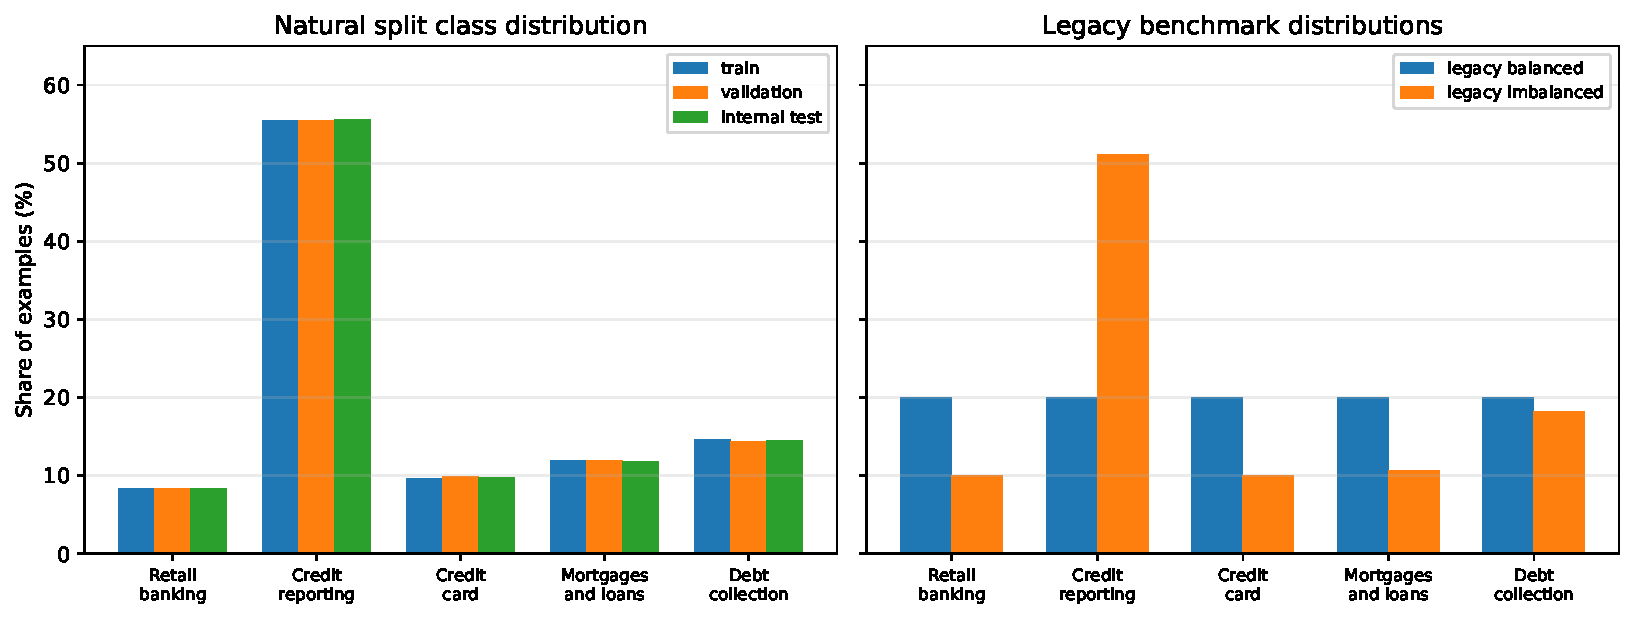
\includegraphics[width=0.74\linewidth]{figures/class_distribution.pdf}
\caption{Class distribution in the leakage-controlled natural splits and in the preserved legacy benchmark subsets. The balanced legacy subsets control class priors, while the imbalanced subsets test deployment-like behaviour under natural prevalence.}
\label{fig:class-distribution}
\end{center}
\end{figure}

The use of both balanced and imbalanced legacy subsets is deliberate. Balanced subsets prevent the majority class from dominating aggregate scores and make class-specific weaknesses easier to detect. Imbalanced subsets preserve a more realistic prevalence pattern and therefore test whether improvements remain useful under deployment-like class priors. Reporting both views is important because a model can appear strong on an imbalanced set by favouring \texttt{credit\_reporting}, while still performing poorly on minority or semantically overlapping categories such as \texttt{debt\_collection}.

Complaint narratives are mostly short to medium length but have a long tail. The median narrative length is 365 characters and the 90th percentile is 1,261 characters. A 500-character training narrative limit fully covers 63.01\% of examples, while 98.90\% of examples are below 512 whitespace tokens. Figure~\ref{fig:lengths} summarises the character and approximate sequence-length distributions. The character limit was selected to keep QLoRA training feasible on 16 GB V100 GPUs while retaining the central complaint signal for the majority of records.

\begin{figure}[tbh]
\begin{center}
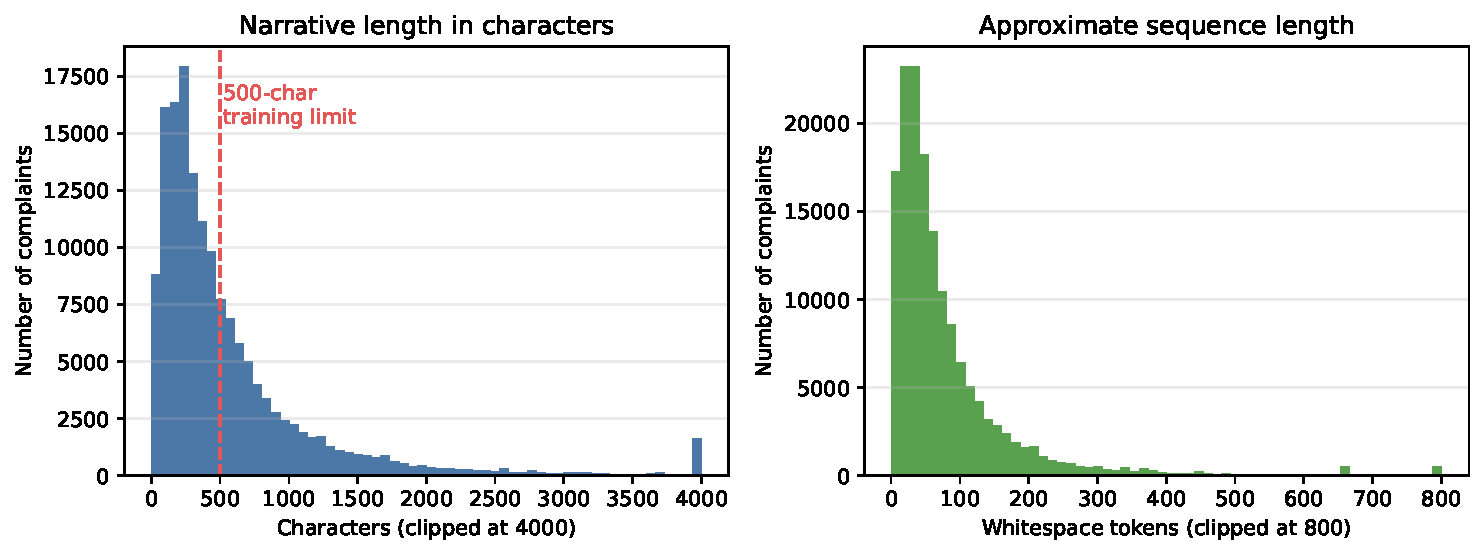
\includegraphics[width=0.92\linewidth]{figures/narrative_length_histogram.pdf}
\caption{Narrative length distribution in the leakage-controlled train/validation/internal-test pool. The left panel shows character length with the 500-character fine-tuning limit; the right panel shows approximate whitespace-token length.}
\label{fig:lengths}
\end{center}
\end{figure}

\subsection{Leakage-controlled split}

To prevent evaluation leakage, the legacy subsets are first removed from the train/validation/internal-test pool. Narrative normalisation applies NFKC Unicode decomposition, whitespace stripping, and lowercasing; a SHA-256 hash of the normalised text is used as a deduplication key. Matching the 12,000 legacy rows (5,909 unique label--narrative pairs) back to the 162,405-row corpus excludes 8,123 rows from the fine-tuning pool through four mechanisms: (1) 4,990 exact normalised-text matches, (2) 3,096 matches where the first 250 normalised characters of a main-corpus narrative equal a legacy narrative truncated at 250 characters, (3) 23 rows whose normalised narrative belongs to the same duplicate group as a matched row but was not itself matched, and (4) 14 cross-label 250-character prefix matches where the main-corpus narrative begins with the same text as a legacy narrative from a different product category. The 250-character threshold is used because it is the minimum truncation length among the legacy subsets, making it a conservative prefix-matching rule that also protects the 500-character legacy variants. These four mechanisms ensure that training data cannot leak any textual prefix of a legacy evaluation record, regardless of label or narrative length.

After legacy exclusion, the remaining pool contains 154,282 rows and 119,583 unique normalised narratives. The split is performed with a fixed seed of 42 and an 80/10/10 ratio, resulting in 123,427 training records, 15,427 validation records, and 15,428 internal test records. The split assigns all rows sharing the same normalised narrative to the same partition, preventing any information leakage between train, validation, and test sets even when narratives appear under different product labels. Duplicate-aware overlap checks confirm zero shared normalised narratives across all three partitions. Exact legacy hashes are also absent from the remaining pool. Legacy examples are therefore retained only for final paired benchmark evaluation.

\subsection{Models}

Two 8B-class open-source model families are used: Qwen3-8B, representing the Qwen3 model family \cite{yang2025qwen3}; and Llama 3.1-8B Instruct, representing the Llama 3 family of open-weight models \cite{dubey2024llama}.
Both models are evaluated as base zero-shot classifiers and as QLoRA fine-tuned classifiers. The base and fine-tuned evaluations use the same prompt format, label set, narrative truncation length, quantisation setup, and decoding strategy.

\subsection{Classical and encoder supervised baselines}

To provide non-LLM reference points, two families of supervised baselines are trained under the same leakage-controlled split and the same 500-character narrative truncation.

\textbf{TF-IDF + Logistic Regression.} The TF-IDF representation uses unigram and bigram features, Unicode accent stripping, sublinear term frequency, minimum document frequency of 2, and a maximum of 200,000 features. Logistic Regression is trained with balanced class weights, $C=2.0$, and a maximum of 2000 iterations. Two budgets are evaluated: a 10,000-example natural training sample matching the QLoRA fixed-budget setting, and the full 123,427-example training split.

\textbf{Fine-tuned transformer encoders.} Three encoder-only models are fine-tuned on the same 10{,}000-example natural training budget used for QLoRA: BERT-base-uncased \cite{devlin2019bert}, DistilBERT-base-uncased \cite{sanh2019distilbert}, and RoBERTa-base \cite{liu2019roberta}. Each model is fine-tuned on TRUBA for 2 epochs with a learning rate of $2\times10^{-5}$, effective batch size 16, linear warm-up over 6\% of steps, and maximum sequence length of 512 tokens. These settings are selected as conservative, commonly used full fine-tuning settings for pretrained encoder models: unlike QLoRA, encoder fine-tuning updates the pretrained encoder weights directly, so a smaller learning rate is used to reduce the risk of destabilising the learned representations; the two-epoch budget and effective batch size 16 mirror the fixed-budget design used for QLoRA; and 512 tokens is the standard maximum input length supported by BERT-style encoders. The 500-character narrative truncation is applied before tokenisation to match the QLoRA setup. All encoder baselines use seed 42 and are evaluated on the internal test set and all 12 legacy subsets under the same metrics as the QLoRA experiments. These baselines fill the gap between simple lexical classifiers and decoder-based LLMs and provide a supervised encoder reference under the same fixed training budget.

\subsection{Prompt and training format}

The same chat-style classification prompt is used for zero-shot inference, QLoRA training, validation inference, internal testing, and legacy evaluation. The prompt follows the model-agnostic five-label JSON-output template used by Roumeliotis et al. for zero-shot CFPB complaint classification \cite{roumeliotis2025think}. Their prompt-engineering discussion motivates this design by noting that structured JSON output is more token-efficient than XML-style formatting, easier to parse consistently across different LLMs, and helpful for constraining predictions to a predefined label set. This is directly relevant to the present study because off-label outputs are operational failures in complaint-routing systems.

The operational prompt template used in this study is:

\begin{quote}
\small
\noindent \textbf{System:} You are an AI assistant specializing in consumer complaint classification. Classify each complaint into exactly one of these categories:
retail\_banking, credit\_reporting, credit\_card, mortgages\_and\_loans, and debt\_collection. Return only valid JSON in this format:
\{"product": "chosen\_category\_name"\}. Do not provide explanations.

\medskip
\noindent \textbf{User:} Complaint:\\
\texttt{[NARRATIVE]}
\end{quote}

Thus, the system message specifies the five allowed categories and enforces a single JSON field, while the user message contains the prefix \texttt{Complaint:} followed by the truncated complaint narrative.

For QLoRA training, each example is converted into a prompt--completion pair. The prompt contains the system and user messages, while the completion contains only the target JSON object with the correct product label, followed by the tokenizer end-of-sequence token. Training uses completion-only loss, so the optimisation target is the label-bearing assistant completion rather than the prompt text. No auxiliary format penalty or special JSON-specific loss is used. During inference, generated text is parsed with a constrained regular expression over the \texttt{product} field; outputs outside the five-label taxonomy are counted as off-label predictions. No retry prompting, synonym normalisation, or external constrained-decoding API is used, so the off-label analysis reflects strict raw model compliance under the fixed prompt.

\subsection{Fine-tuning protocol}

Qwen3-8B is used as the primary model for validation-based protocol selection. The goal of this stage is not exhaustive hyperparameter optimisation, but a limited fixed-budget protocol selection that can be applied unchanged to a second model family. Table~\ref{tab:protocol-selection} summarises the Qwen3-8B validation experiments used to choose the final protocol. The best validation macro-F1 is obtained with natural sampling, learning rate $2\times10^{-4}$, LoRA rank 16, and two epochs. Balanced sampling improves some minority-class behaviour in the one-epoch trials but does not improve overall validation macro-F1 after the second-stage comparison.

\begin{table}[h!]
\caption{Validation-stage protocol selection on Qwen3-8B. The selected final protocol is natural sampling, $2\times10^{-4}$ learning rate, LoRA rank 16, and two epochs.}
\label{tab:protocol-selection}
\begin{center}
\begin{tabular}{llrrrrr}
\hline
Experiment & Sampling & LR & Rank & Epochs & Macro-F1 & Debt F1\\
\hline
Qwen3-8B pilot & natural & $2\times10^{-4}$ & 16 & 1 & 0.8098 & 0.6429 \\
Qwen3-8B balanced E1 & balanced & $2\times10^{-4}$ & 16 & 1 & 0.8040 & 0.6667 \\
Qwen3-8B balanced E2 & balanced & $1\times10^{-4}$ & 16 & 1 & 0.7948 & 0.6552 \\
Qwen3-8B balanced E3 & balanced & $2\times10^{-4}$ & 8 & 1 & 0.7951 & 0.6574 \\
Qwen3-8B natural 2-epoch & natural & $2\times10^{-4}$ & 16 & 2 & 0.8235 & 0.7033 \\
Qwen3-8B balanced 2-epoch & balanced & $2\times10^{-4}$ & 16 & 2 & 0.8065 & 0.6456 \\

\end{tabular}
\end{center}
\end{table}

The final protocol is fixed as follows: natural training sampling; 10,000 training examples; 2,000 validation examples; two epochs; learning rate $2 \times 10^{-4}$; LoRA rank/alpha 16/32; maximum narrative length of 500 characters; maximum input length of 512 tokens; seeds 42, 43, and 44.
The 10,000-example training budget is a deliberate fixed-compute design choice. The full training split contains 123,427 records, but training all models on the full split would substantially increase the computational burden of the three-seed, two-model protocol on 16 GB V100 GPUs. By using the same 10,000-example natural sample, 2,000-example validation sample, and two-epoch budget for each seed and model, the study prioritises a reproducible paired comparison over maximum possible leaderboard performance. Consequently, the reported QLoRA scores should be interpreted as fixed-budget adaptation results rather than upper-bound performance estimates. Larger training budgets may improve absolute scores and are therefore treated as future work rather than as part of the present controlled evaluation.

The same frozen protocol is then applied to Llama 3.1-8B without additional hyperparameter search. This design treats Llama 3.1-8B as a confirmatory model rather than a separately optimised model: the objective is to test whether the selected protocol transfers across model families, not to maximise the score of each model through model-specific tuning.

\subsection{Experimental setup}

All experiments were conducted on the TRUBA ARF high-performance computing infrastructure. Training and inference jobs were submitted with SLURM on the \texttt{akya-cuda} partition using one NVIDIA Tesla V100-SXM2 GPU with 16 GB memory and 10 CPU cores per job. The software environment used Python 3.10.20, PyTorch 2.7.1 with CUDA 11.8 wheels, Transformers, PEFT, TRL, bitsandbytes 0.46.1, pandas, and scikit-learn. Models were stored on shared scratch storage and loaded from local Hugging Face checkpoints in offline mode during SLURM jobs. QLoRA training used 4-bit NF4 quantisation with double quantisation and FP16 compute; QLoRA jobs used batch size 1 with gradient accumulation 16. Encoder fine-tuning used batch size 4 with gradient accumulation 4, giving the same effective batch size of 16. Final LLM inference used greedy decoding, maximum 32 generated tokens, batch size 1, and constrained JSON-style prompting with a fixed five-label taxonomy.

\subsection{Evaluation and statistical analysis}

The primary metrics are accuracy, macro-F1, and weighted F1. Macro-F1 is emphasised because the natural CFPB distribution is class-imbalanced. Class-level F1 is also reported, with particular attention to \texttt{debt\_collection}. Internal test confidence intervals are estimated using 300 bootstrap resamples over archived prediction files. Legacy benchmark gains are evaluated with one-sided Wilcoxon signed-rank tests over the 12 paired legacy subsets, comparing base zero-shot scores with the mean fine-tuned score across the three seeds. A non-parametric paired test is used because the legacy benchmark contains only 12 subset-level observations and normality should not be assumed. The alternative hypothesis is directional because the experimental question is whether QLoRA fine-tuning improves over base zero-shot inference under the same model family and evaluation pipeline. Inference latency is measured as wall-clock generation time per example during the prediction loop, excluding model loading time, and is reported as mean seconds per example; it should therefore be interpreted as serial batch-size-1 latency rather than optimised batched throughput.

\section{Results}

\subsection{Internal test performance}

Table~\ref{tab:internal-summary} shows the internal test results on the leakage-controlled held-out split. Both model families show large gains from QLoRA fine-tuning. Qwen3-8B improves from 0.6294 to 0.8350 macro-F1, a gain of 0.2056, while Llama 3.1-8B improves from 0.6189 to 0.8378 macro-F1, a gain of 0.2189. Weighted F1 also increases substantially, from 0.7202 to 0.8686 for Qwen3-8B and from 0.7094 to 0.8705 for Llama 3.1-8B. The fact that macro-F1 and weighted F1 both improve is important: the models do not merely become better at the majority \texttt{credit\_reporting} class, but also improve the balance of performance across the five-class taxonomy.

The class-level pattern in Table~\ref{tab:internal-summary} is particularly relevant for the central complaint-triage problem. After fine-tuning, \texttt{debt\_collection} F1 reaches 0.7546 for Qwen3-8B and 0.7613 for Llama 3.1-8B. This category is operationally important because debt collection narratives frequently mention disputed accounts, credit bureaus, and credit reports, making them easy to confuse with \texttt{credit\_reporting}. The internal test results therefore support the main claim of the paper: QLoRA fine-tuning teaches the open-source LLMs the dataset-specific decision boundary that zero-shot prompting alone does not capture reliably.

\begin{table}[h!]
\caption{Internal test summary. Fine-tuned scores are mean$\pm$sample standard deviation over seeds 42, 43, and 44.}
\label{tab:internal-summary}
\begin{center}
\footnotesize
\begin{tabular*}{\textwidth}{@{\extracolsep{\fill}}lrrrrrrr}
\hline
Model & Base macro-F1 & FT macro-F1 & Gain & Base wF1 & FT wF1 & Gain & FT debt F1\\
\hline
Qwen3-8B & 0.6294 & 0.8350$\pm$0.0017 & 0.2056 & 0.7202 & 0.8686$\pm$0.0011 & 0.1483 & 0.7546$\pm$0.0046 \\
Llama 3.1-8B & 0.6189 & 0.8378$\pm$0.0026 & 0.2189 & 0.7094 & 0.8705$\pm$0.0011 & 0.1611 & 0.7613$\pm$0.0072 \\

\end{tabular*}
\end{center}
\end{table}

Bootstrap confidence intervals confirm that the internal-test gains are well separated from zero for both models (Table~\ref{tab:bootstrap-ci}). Each cell in Table~\ref{tab:bootstrap-ci} reports the point estimate followed by its 95\% bootstrap confidence interval in brackets. For Qwen3-8B, the macro-F1 gain is 0.2060 with a 95\% confidence interval of [0.1965, 0.2143]. For Llama 3.1-8B, the macro-F1 gain is 0.2191 with a 95\% confidence interval of [0.2099, 0.2266]. Accuracy and weighted-F1 gains are similarly positive for both models. These intervals are narrow because the internal test set contains 15,428 examples, and none of the gain intervals approaches zero. Thus, the observed improvement is not a small fluctuation caused by a favourable sample; it is a stable effect at the prediction level.

\begin{table}[h!]
\caption{Bootstrap 95\% confidence intervals on the internal test. Each cell reports point estimate [lower, upper]. Fine-tuned scores are seed means, gain is fine-tuned minus base, and confidence intervals are estimated from 300 bootstrap resamples over archived prediction files.}
\label{tab:bootstrap-ci}
\begin{center}
\begin{tabular}{llrrr}
\hline
Model & Metric & Base & Fine-tuned & Gain\\
\hline
Qwen3-8B & accuracy & 0.7351 [0.7287, 0.7411] & 0.8697 [0.8648, 0.8745] & 0.1346 [0.1285, 0.1402] \\
Qwen3-8B & macro-F1 & 0.6289 [0.6201, 0.6385] & 0.8350 [0.8288, 0.8421] & 0.2060 [0.1965, 0.2143] \\
Qwen3-8B & weighted F1 & 0.7201 [0.7119, 0.7280] & 0.8685 [0.8641, 0.8735] & 0.1484 [0.1409, 0.1555] \\
Llama 3.1-8B & accuracy & 0.7319 [0.7254, 0.7391] & 0.8716 [0.8667, 0.8763] & 0.1397 [0.1336, 0.1457] \\
Llama 3.1-8B & macro-F1 & 0.6187 [0.6094, 0.6282] & 0.8378 [0.8313, 0.8440] & 0.2191 [0.2099, 0.2266] \\
Llama 3.1-8B & weighted F1 & 0.7094 [0.7014, 0.7169] & 0.8704 [0.8656, 0.8744] & 0.1610 [0.1534, 0.1684] \\

\end{tabular}
\end{center}
\end{table}

\subsection{Seed stability}

Seed stability is evaluated by repeating the final QLoRA protocol three times for each model family, using seeds 42, 43, and 44. The train/validation/internal-test split, 10,000-example training budget, validation set, prompt template, learning rate, LoRA configuration, number of epochs, and final evaluation sets are kept fixed. The random seed affects the stochastic parts of fine-tuning, including training-order shuffling, adapter initialisation, dropout, and low-level GPU randomness where applicable. Each seed-specific adapter is then evaluated on the same internal test set, and the mean and standard deviation of each metric are computed across the three independently fine-tuned adapters.

Across these per-seed internal test runs, macro-F1 sample standard deviation is 0.0017 for Qwen3-8B and 0.0026 for Llama 3.1-8B, indicating that the fine-tuning protocol is highly reproducible and not dependent on a single favourable random seed. Weighted F1 and accuracy show similarly tight dispersion, remaining close to approximately 0.001 across both model families. The largest per-seed spread is observed for debt-collection F1 (0.0046 for Qwen3-8B; 0.0072 for Llama 3.1-8B), which reflects the inherent difficulty of that class boundary rather than training instability.

\subsection{Legacy benchmark performance}

Table~\ref{tab:legacy-summary} summarises performance over the 12 preserved legacy subsets. These subsets were created before the fine-tuning experiments and were excluded from fine-tuning, validation, and protocol selection. They therefore act as an external continuity benchmark connecting the zero-shot setting to the fine-tuned setting without contaminating the training data. The average macro-F1 gain is 0.1853 for Qwen3-8B and 0.2289 for Llama 3.1-8B. Weighted F1 also increases by 0.1676 and 0.2070, respectively.

The legacy benchmark is important because it tests whether the internal-test gains survive a different evaluation construction. Unlike the internal test, the legacy benchmark contains both balanced and imbalanced subsets. The balanced subsets expose class-level weaknesses that can be hidden by majority-class prevalence, while the imbalanced subsets test a more natural complaint distribution. The gains in Table~\ref{tab:legacy-summary} show that fine-tuning improves performance across this mixed benchmark rather than overfitting to a single natural split.

\begin{table}[h!]
\caption{Legacy benchmark summary across 12 preserved zero-shot subsets. Fine-tuned scores are averaged over three seeds and all legacy subsets.}
\label{tab:legacy-summary}
\begin{center}
\begin{tabular}{lrrrrrr}
\hline
Model & Base macro-F1 & FT macro-F1 & Gain & Base wF1 & FT wF1 & Gain\\
\hline
Qwen3-8B & 0.6150 & 0.8003 & 0.1853 & 0.6486 & 0.8163 & 0.1676 \\
Llama 3.1-8B & 0.5763 & 0.8053 & 0.2289 & 0.6134 & 0.8204 & 0.2070 \\

\end{tabular}
\end{center}
\end{table}

The paired Wilcoxon tests in Table~\ref{tab:wilcoxon} show that the fine-tuned models consistently outperform their base zero-shot counterparts over the 12 legacy subsets. For each model and metric, the one-sided $p$ value is 0.000244. Since there are 12 paired subsets, this result indicates that the improvement is directionally consistent across the preserved benchmark rather than being driven by one or two favourable subsets. The rank-biserial effect size is 1.000 for every model--metric pair because all 12 paired differences are positive. The median gains are close to the mean gains for all three metrics, which further suggests that the improvement is not dominated by an outlier subset. For example, Qwen3-8B has a mean macro-F1 gain of 0.1853 and a median macro-F1 gain of 0.1842, while Llama 3.1-8B has a mean macro-F1 gain of 0.2289 and a median macro-F1 gain of 0.2217.

\begin{table}[h!]
\caption{One-sided Wilcoxon signed-rank tests over 12 legacy subsets. The alternative hypothesis is that fine-tuned performance is greater than base zero-shot performance. Effect size is the matched-pairs rank-biserial correlation.}
\label{tab:wilcoxon}
\begin{center}
\begin{tabular}{llrrrrrr}
\hline
Model & Metric & Base mean & FT mean & Mean gain & Median gain & Effect & $p$\\
\hline
Qwen3-8B & accuracy & 0.6593 & 0.8160 & 0.1566 & 0.1533 & 1.000 & 0.0002441 \\
Qwen3-8B & macro-F1 & 0.6150 & 0.8003 & 0.1853 & 0.1842 & 1.000 & 0.0002441 \\
Qwen3-8B & weighted F1 & 0.6486 & 0.8163 & 0.1676 & 0.1670 & 1.000 & 0.0002441 \\
Llama 3.1-8B & accuracy & 0.6394 & 0.8201 & 0.1807 & 0.1835 & 1.000 & 0.0002441 \\
Llama 3.1-8B & macro-F1 & 0.5763 & 0.8053 & 0.2289 & 0.2217 & 1.000 & 0.0002441 \\
Llama 3.1-8B & weighted F1 & 0.6134 & 0.8204 & 0.2070 & 0.2089 & 1.000 & 0.0002441 \\

\end{tabular}
\end{center}
\end{table}

\subsection{Supervised baseline comparison}

Table~\ref{tab:supervised-baselines} reports the TF-IDF + Logistic Regression and fine-tuned encoder baselines. With the same 10,000-example training budget used for QLoRA, TF-IDF + Logistic Regression reaches 0.8021 internal macro-F1 and 0.7965 mean legacy macro-F1. Under the same 10,000-example budget, BERT-base and RoBERTa-base reach almost identical internal macro-F1 scores of 0.8036, while DistilBERT reaches 0.7950. When TF-IDF + Logistic Regression is trained on the full 123,427-example training split, it reaches 0.8345 internal macro-F1 and 0.8279 legacy macro-F1, matching or exceeding the fine-tuned LLMs on aggregate supervised classification scores. These results show that classical and encoder baselines remain strong for a stable five-label taxonomy, while the QLoRA-tuned decoder models provide the paired zero-shot-to-fine-tuned comparison and prompt-controllable operation studied in this paper.

\begin{table}[H]
\caption{Supervised baselines under the leakage-controlled split. TF-IDF variants use 500-character truncation; encoder models use a 10,000-example budget, 2 epochs, effective batch size 16, seed 42, 512-token maximum sequence length, and 500-character truncation. Legacy scores are averages over the 12 preserved subsets.}
\label{tab:supervised-baselines}
\begin{center}
\begin{tabular*}{\textwidth}{@{\extracolsep{\fill}}lrrrrr}
\hline
Baseline & Train examples & Internal macro-F1 & Internal wF1 & Legacy macro-F1 & Debt F1\\
\hline
TF-IDF+LR 10k & 10000 & 0.8021 & 0.8404 & 0.7965 & -- \\
TF-IDF+LR full & 123427 & 0.8345 & 0.8655 & 0.8279 & -- \\
BERT-base & 5000 & 0.7757 & 0.8270 & 0.7358 & 0.6691 \\
DistilBERT & 5000 & 0.7548 & 0.8132 & 0.7122 & 0.6600 \\
RoBERTa-base & 5000 & 0.7864 & 0.8332 & 0.7520 & 0.6943 \\

\end{tabular*}
\end{center}
\end{table}

The comparison clarifies the scope of the paper. The claim is not that QLoRA-tuned LLMs universally dominate supervised classifiers for a fixed taxonomy. Rather, locally deployable open-source LLMs can be moved from weaker zero-shot performance to a competitive supervised-classification regime using a fixed 10,000-example PEFT budget, while preserving the same promptable model family for zero-shot and fine-tuned operation. Encoder models produce deterministic categorical outputs without JSON parsing and are computationally efficient; decoder LLMs require more compute but support zero-shot inference, prompt constraints, and potential label redefinition without retraining. The full-data TF-IDF result also indicates that simple lexical models remain attractive when the taxonomy is fixed and all labelled data can be used. In this sense, the classical baselines are not treated as weak straw-man competitors; they define a practical efficiency reference. If the deployment objective is only to classify a stable five-label taxonomy with abundant labelled data, TF-IDF or encoder models may be preferable. The value of the LLM/QLoRA pipeline is instead in the paired zero-shot-to-adapted workflow, local open-weight deployment, and reuse of the same instruction-following model when taxonomies, prompts, or downstream routing requirements change.

\subsection{Error analysis}

Figure~\ref{fig:confusion-matrices} reports row-normalised internal-test confusion matrices for both model families, comparing the base zero-shot models with the fine-tuned means across three seeds. The diagonal cells become darker after fine-tuning, indicating improved within-class recall across the five-category taxonomy. The dominant zero-shot error is the confusion of \texttt{debt\_collection} with \texttt{credit\_reporting}: Qwen3-8B makes this error 1,235 times in zero-shot mode and 424.7 times after fine-tuning on average, a reduction of approximately 66\%; Llama 3.1-8B makes the same error 1,401 times in zero-shot mode and 435.7 times after fine-tuning, a reduction of approximately 69\%. This explains the large class-level F1 gains for \texttt{debt\_collection} reported in Table~\ref{tab:internal-summary}.

The largest visual change occurs in the \texttt{debt\_collection} row: Qwen3-8B increases the correct debt-collection proportion from 32.5\% in zero-shot mode to 73.4\% after QLoRA fine-tuning, while Llama 3.1-8B increases it from 20.7\% to 73.1\%. Fine-tuning also reduces several other high-frequency confusions. For Qwen3-8B, \texttt{retail\_banking} $\rightarrow$ \texttt{credit\_card} decreases from 561.0 to 90.3. For Llama 3.1-8B, \texttt{mortgages\_and\_loans} $\rightarrow$ \texttt{credit\_reporting} decreases from 339.0 to 207.7, \texttt{credit\_reporting} $\rightarrow$ \texttt{credit\_card} decreases from 312.0 to 126.3, and \texttt{retail\_banking} $\rightarrow$ \texttt{credit\_card} decreases from 333.0 to 83.0. These reductions suggest that the adapters are not only memorising one problematic class but are reshaping several neighbouring decision boundaries in the financial taxonomy.

One residual issue remains visible in both models: after fine-tuning, credit reporting to debt collection becomes one of the largest remaining confusions. This is an expected trade-off when the model becomes less conservative about assigning debt collection labels; it improves recall for \texttt{debt\_collection} but still leaves a boundary that should be studied in future class-specific prompting or cost-sensitive training. The figure also shows why the problem is difficult: the strongest remaining off-diagonal cells are still between \texttt{debt\_collection}, \texttt{credit\_reporting}, and \texttt{mortgages\_and\_loans}, categories that often co-occur in consumer narratives about disputed debts, credit reports, and loan servicing. The full top-confusion counts are retained with the archived analysis outputs for reproducibility.

\begin{figure}[t]
\begin{center}
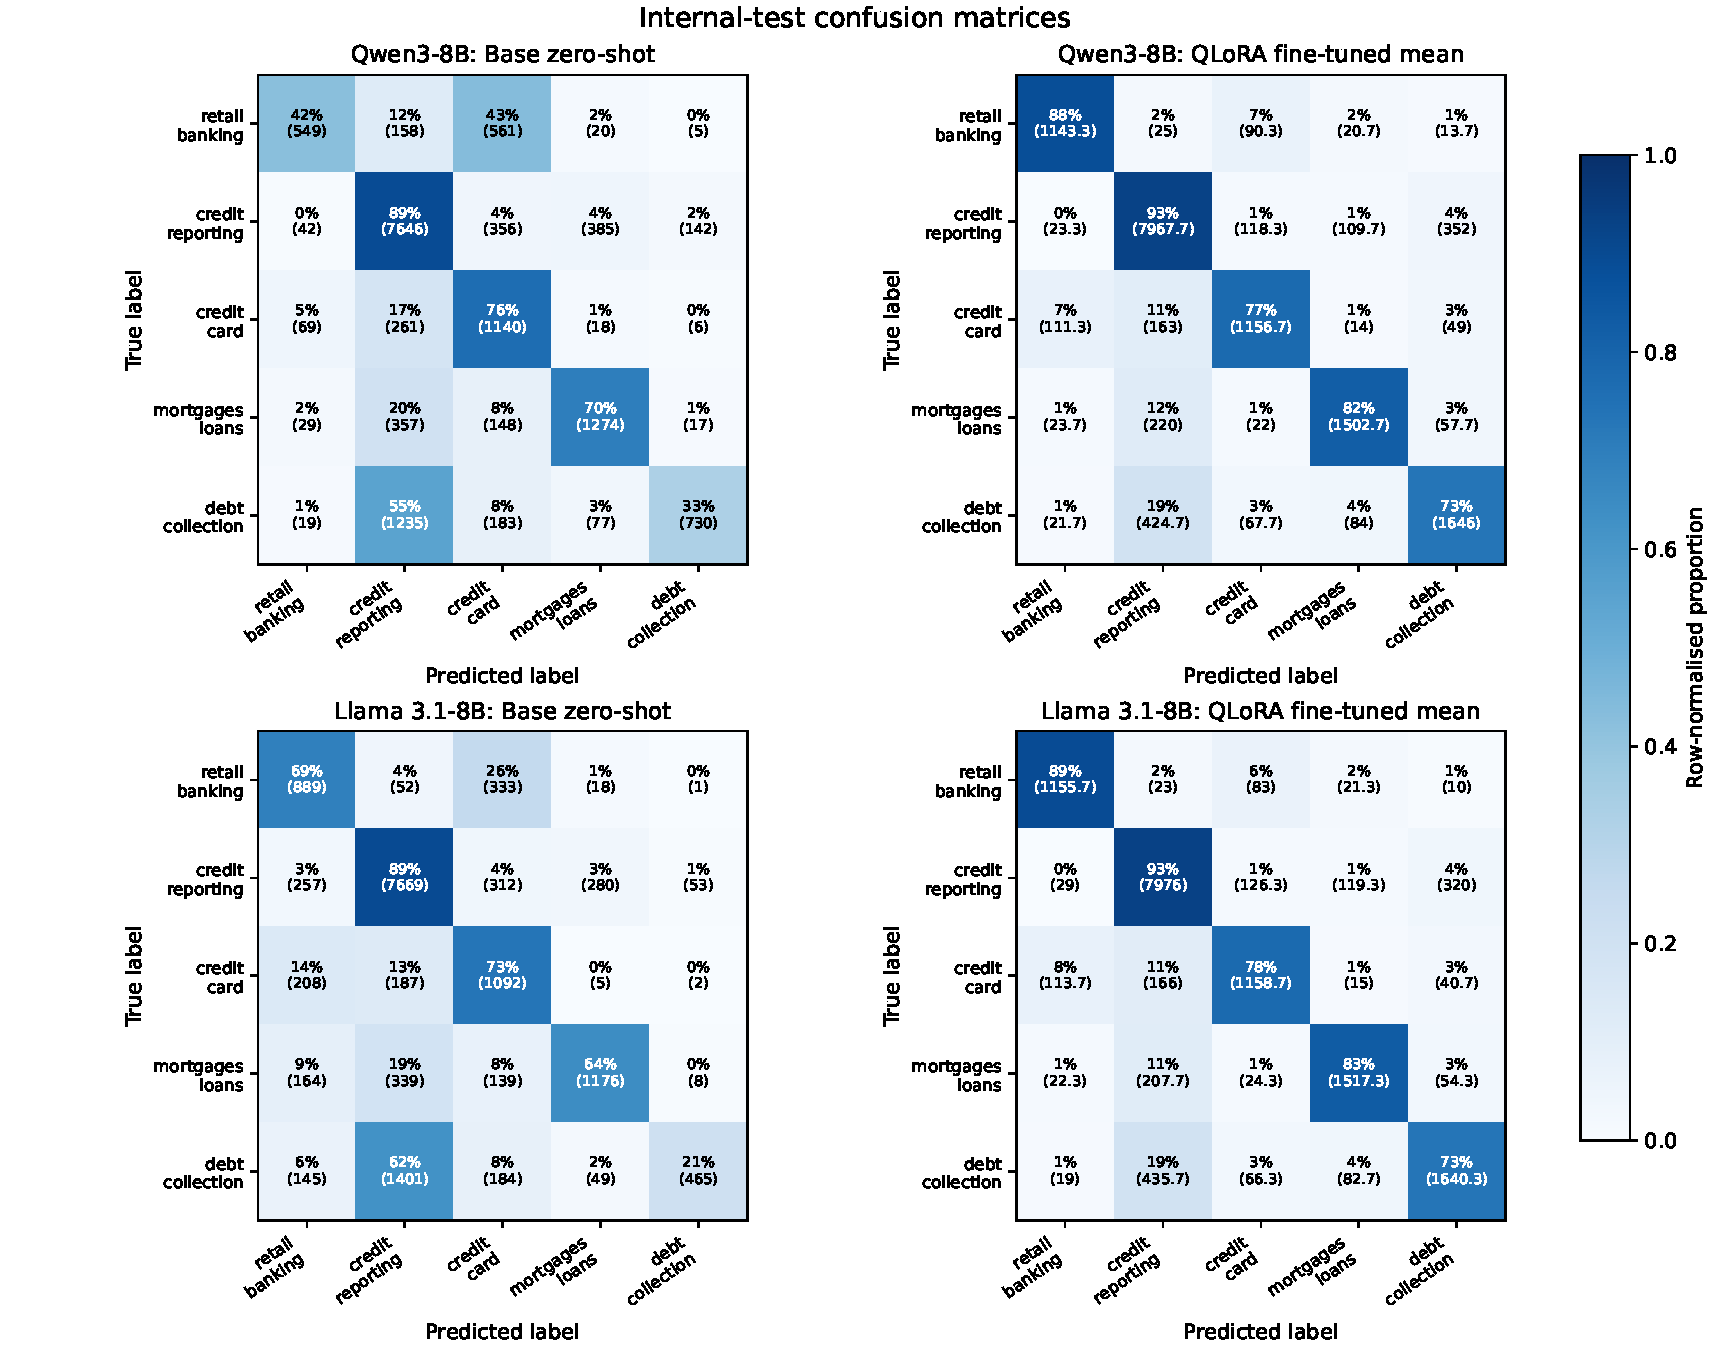
\includegraphics[width=0.98\linewidth]{figures/internal_confusion_matrices.pdf}
\caption{Row-normalised internal-test confusion matrices for base zero-shot and QLoRA fine-tuned models. Fine-tuned matrices are averaged over seeds 42, 43, and 44; cell annotations show row percentage and count.}
\label{fig:confusion-matrices}
\end{center}
\end{figure}

\subsection{Latency}

Fine-tuning increases inference latency because adapter-based inference is slower than base-only generation in this setup. On the internal test set, Qwen3-8B latency increases from 0.603 to 0.912 seconds per complaint, a delta of 0.309 seconds. Llama 3.1-8B latency increases from 0.487 to 0.808 seconds, a delta of 0.321 seconds.

This latency result is important for deployment interpretation. The additional cost is measurable, but it is modest relative to the accuracy and macro-F1 gains in Tables~\ref{tab:internal-summary} and~\ref{tab:legacy-summary}. In an offline regulatory analytics workflow or a semi-real-time complaint-routing system, an additional one third of a second per complaint is likely acceptable if it reduces high-impact class confusions such as \texttt{debt\_collection} $\rightarrow$ \texttt{credit\_reporting}. For strict real-time systems, however, these latency deltas indicate that throughput planning and batching would be necessary.

\subsection{Off-label output rates}

Off-label predictions are defined as generated outputs that cannot be parsed to any of the five allowed product categories. Both base and fine-tuned models produce near-zero off-label rates. For Qwen3-8B, the base model generates one off-label prediction across 15,428 internal-test examples (0.006\%), while all three fine-tuned seeds produce zero off-label outputs. For Llama 3.1-8B, the base model produces zero off-label predictions on the internal test, and one isolated off-label output appears in seed 42 of the fine-tuned model (0.002\% across 46,284 seed-examples). On the 12 legacy subsets, neither base nor fine-tuned models of either family produce any off-label predictions. These results confirm that the constrained JSON-output prompt format and greedy decoding reliably keep both base and fine-tuned models within the allowed label taxonomy, and that fine-tuning does not introduce taxonomy violations.

\section{Discussion}

The results show that PEFT substantially improves open-source LLM complaint classification under a leakage-safe evaluation protocol. The evidence is deliberately layered. Figure~\ref{fig:class-distribution} first establishes that the task is not a balanced toy problem: the natural data are dominated by \texttt{credit\_reporting}, while the legacy benchmark intentionally contains both balanced and imbalanced views. Figure~\ref{fig:lengths} then shows that the complaints are mostly short enough for efficient 8B-model adaptation on a 16 GB GPU, but still contain a long tail that motivates explicit truncation and reproducible preprocessing. These dataset figures are therefore not merely descriptive; they justify the evaluation design and the use of macro-F1, class-level analysis, and balanced/imbalanced legacy subsets.

Tables~\ref{tab:internal-summary} and~\ref{tab:bootstrap-ci} provide the internal-test evidence. The macro-F1 gains of 0.2056 for Qwen3-8B and 0.2189 for Llama 3.1-8B are large enough to be practically meaningful, and the bootstrap intervals for both model families show that the prediction-level improvement is statistically stable. This matters because a fine-tuning paper can otherwise be criticised for reporting only a single aggregate score without uncertainty. Here, the internal-test evidence indicates that the gain is both large and precise.

Tables~\ref{tab:legacy-summary} and~\ref{tab:wilcoxon} provide the second layer of evidence. The preserved legacy subsets are not used for training or model selection, so they test whether the fine-tuned models generalise back to the earlier zero-shot benchmark setting. The Wilcoxon results show that the gains are paired and consistent across all 12 legacy subsets and across accuracy, macro-F1, and weighted F1. This is the methodological bridge of the paper: the study does not simply replace a zero-shot experiment with a fine-tuned experiment; it reuses the legacy subsets as protected final benchmarks and shows that the improvement survives that bridge.

Table~\ref{tab:supervised-baselines} adds an important reference point. Well-configured TF-IDF and encoder models remain strong supervised baselines for this fixed five-class taxonomy. This prevents overclaiming: the contribution is not that PEFT always outperforms classical or encoder-based supervised learning, but that it provides a leakage-controlled and locally deployable path from zero-shot open-source LLM inference to competitive supervised performance under a fixed training budget.

Figure~\ref{fig:confusion-matrices} explains where the improvement comes from. The strongest practical improvement is observed for \texttt{debt\_collection}. In zero-shot mode, both models over-map debt collection narratives to \texttt{credit\_reporting}; this is plausible because consumer debt disputes often mention credit reports, credit bureaus, disputed accounts, and collections simultaneously. Fine-tuning reduces this dominant error by approximately two thirds in both model families, indicating that the adapters learn a more dataset-specific boundary between credit reporting and debt collection. The remaining \texttt{credit\_reporting} $\rightarrow$ \texttt{debt\_collection} errors also reveal where future work should focus: class-boundary calibration rather than only global accuracy improvement.

The latency analysis adds the deployment trade-off. The fine-tuned models are slower by approximately 0.31--0.32 seconds per complaint, but the gain is large enough to make this trade-off favourable for offline analytics, audit, compliance, or semi-real-time routing. This discussion is important because it prevents the paper from presenting F1 improvements in isolation. In realistic complaint-processing systems, accuracy, latency, reproducibility, and data governance must be evaluated together.

The results should also be interpreted with appropriate deployment safeguards. The study evaluates product-category classification rather than automated consumer-facing decisions, and it does not use demographic attributes or attempt to infer protected characteristics. Nevertheless, class-specific error disparities can still matter operationally because routing errors may delay responses to particular complaint types. The confusion-matrix analysis therefore functions as a limited bias and reliability audit at the product-category level: it shows that fine-tuning reduces the largest \texttt{debt\_collection} $\rightarrow$ \texttt{credit\_reporting} error, but it also identifies the remaining credit-reporting/debt-collection boundary as a candidate for human review, cost-sensitive training, or class-specific calibration in deployment.

The study also illustrates why leakage control matters. If the legacy zero-shot subsets had been allowed into training, the paired benchmark comparison in Tables~\ref{tab:legacy-summary} and~\ref{tab:wilcoxon} would have been contaminated. By excluding them before split construction and using them only at final evaluation, the present work preserves the interpretability of the legacy comparison. This leakage-safe design is also what makes the comparison with prior zero-shot CFPB studies meaningful: the paper evaluates the transition from zero-shot inference to QLoRA fine-tuning without erasing the benchmark that motivated the transition.

\section{Limitations}

This study does not propose a new model architecture or a new PEFT algorithm. LoRA and QLoRA are established methods; the contribution is a controlled empirical evaluation in a specific high-value application domain. The experiments use two 8B-class model families and a fixed 10,000-example training budget; larger models (13B--70B parameters) or additional decoder architectures such as Mistral and Mixtral represent a natural extension but are deferred due to the computational burden of the three-seed, two-model evaluation protocol on 16 GB V100 GPUs. The prompt is also fixed rather than optimised. This choice supports comparability with the zero-shot CFPB prompt template used in prior work and keeps the paired base-versus-fine-tuned comparison controlled, but it does not rule out prompt sensitivity. Alternative prompt phrasings, label descriptions, few-shot demonstrations, or constrained decoding could change zero-shot and fine-tuned performance and should be evaluated in future prompt-ablation studies. The 500-character narrative truncation was selected for GPU feasibility and fully covers 63\% of examples, but may discard useful information in the long tail of complaints; ablating this limit at shorter and longer values remains future work. Similarly, the fixed 10,000-example training budget was chosen to enable a controlled paired comparison; mapping the accuracy--compute frontier across larger budgets would further characterise the efficiency of PEFT relative to full-data classical learning and encoder fine-tuning. Encoder-only models could also be further strengthened with domain-adapted checkpoints, hyperparameter searches, and larger encoder variants. Latency measurements are serial batch-size-1 measurements; deployment-oriented batching and throughput analysis are left for future work. The CFPB corpus is English-language and domain-specific, and the present split is not temporal. A temporal split was not used because the primary goal was a paired comparison against preserved legacy zero-shot subsets; robustness to cross-year drift in complaint style, product definitions, or consumer use of generative writing tools remains a separate deployment question. Finally, although the preserved legacy subsets are separated from training and validation, they are still drawn from the same CFPB source distribution rather than from an independently collected external dataset.

\section{Conclusion}

This paper evaluates the transition from zero-shot open-source LLM inference to leakage-controlled QLoRA fine-tuning for consumer complaint classification. Across Qwen3-8B and Llama 3.1-8B, parameter-efficient fine-tuning produces large and stable gains over base zero-shot inference on both an internal test set and preserved legacy zero-shot subsets. The paired design shows that the gain is not merely a result of changing infrastructure, prompts, or evaluation sets; it is observed when the same model families are compared before and after task-specific adaptation under protected data splits. The findings support the use of locally deployable PEFT pipelines for regulated complaint triage settings where commercial API use may be costly, difficult to reproduce, or undesirable for data-governance reasons.

\section*{Acknowledgment and/or disclaimers, if any}

The numerical experiments reported in this study were carried out on the TRUBA ARF high-performance computing infrastructure operated by TÜBİTAK ULAKBİM. The authors gratefully acknowledge the computational resources and technical infrastructure provided by TRUBA.

\section*{Declaration of Generative AI and AI-assisted technologies, if any}

During the preparation of this manuscript, the authors used AI-assisted tools only for English grammar correction, wording refinement, and LaTeX formatting support. The research idea, experimental design, dataset preparation, model fine-tuning, inference runs, statistical analyses, interpretation of results, and final scientific decisions were carried out by the authors. The authors reviewed and edited all AI-assisted text and take full responsibility for the content of the manuscript.

\section*{Data availability statement}

The source CFPB complaint data are publicly available from the Consumer Financial Protection Bureau. The derived split manifests, experiment scripts, classical baseline outputs, and archived metric tables are maintained in a GitHub repository that is currently private. The repository will be made available to reviewers upon request and will be considered for public release after acceptance, subject to anonymisation, repository-cleaning, storage, and model-license requirements.

\section*{Funding, if any}

The authors received no specific funding for this study.

\section*{Conflict of interest, if any}

The authors declare no conflict of interest.

\begin{thebibliography}{99}
\setlength{\itemsep}{1pt}
\setlength{\parsep}{0pt}

\bibitem{devlin2019bert} Devlin J, Chang MW, Lee K, Toutanova K. BERT: pre-training of deep bidirectional transformers for language understanding. In: Proceedings of NAACL-HLT; Minneapolis, MN, USA; 2019. pp. 4171-4186.

\bibitem{bozyigit2022foodcomplaints} Bozyigit F, Dogan O, Kilinc D. Categorization of customer complaints in food industry using machine learning approaches. Journal of Intelligent Systems: Theory and Applications 2022; 5 (1): 85-91.

\bibitem{gewaly2024telecomcomplaint} Gewaly MM, Saeed MS, Ammar AM. Machine learning approach for complaint prediction in the telecom industry. In: 2024 Intelligent Methods, Systems, and Applications; 2024. pp. 12-17.

\bibitem{vairetti2024complaintpriority} Vairetti C, Aranguiz I, Maldonado S, Karmy JP, Leal A. Analytics-driven complaint prioritisation via deep learning and multicriteria decision-making. European Journal of Operational Research 2024; 312 (3): 1108-1118.

\bibitem{raju2022cfpbtopic} Raju SV, Bolla BK, Nayak DK, Jyothsna K. Topic modelling on Consumer Financial Protection Bureau data: an approach using BERT based embeddings. In: Proceedings of IEEE International Conference; 2022.

\bibitem{das2024negative} Das S, Singh A, Saha S, Maurya A. Negative review or complaint? Exploring interpretability in financial complaints. IEEE Transactions on Computational Social Systems 2024; 11 (3): 3606. doi: 10.1109/TCSS.2023.3338357.

\bibitem{shin2025adoption} Shin M, Kim J, Shin J. The adoption and efficacy of large language models: evidence from consumer complaints in the financial industry. arXiv:2311.16466, 2025.

\bibitem{liang2025widespread} Liang W, Zhang Y, Codreanu M, Wang J, Cao H et al. The widespread adoption of large language model-assisted writing across society. arXiv:2502.09747, 2025.

\bibitem{yuan2024framework} Yuan L, Ouyang X, Bai R, Zhu X, Zhou Y et al. A framework for categorizing complaint text via large language model. In: 2024 7th International Conference on Advanced Algorithms and Control Engineering; 2024. doi: 10.1109/ICAACE61206.2024.10549750.

\bibitem{li2025teleeval} Li F, Wang Y, Xu Y, Wang S, Liang J et al. Performance evaluations of large language models for customer service. International Journal of Machine Learning and Cybernetics 2025; 16: 2997-3017. doi: 10.1007/s13042-024-02432-9.

\bibitem{gullu2025complaintllm} Güllü M, Atagün E, Biroğul S, Barışçı N. Customer complaint classification with large language models. In: 2025 International Conference on Artificial Intelligence, Computer, Data Sciences and Applications; Antalya, Türkiye; 2025. doi: 10.1109/ACDSA65407.2025.11166338.

\bibitem{roumeliotis2025think} Roumeliotis KI, Tselikas ND, Nasiopoulos DK. Think before you classify: the rise of reasoning large language models for consumer complaint detection and classification. Electronics 2025; 14: 1070. doi: 10.3390/electronics14061070.

\bibitem{sanh2019distilbert} Sanh V, Debut L, Chaumond J, Wolf T. DistilBERT, a distilled version of BERT: smaller, faster, cheaper and lighter. arXiv:1910.01108, 2019.

\bibitem{liu2019roberta} Liu Y, Ott M, Goyal N, Du J, Joshi M et al. RoBERTa: a robustly optimized BERT pretraining approach. arXiv:1907.11692, 2019.

\bibitem{sy2024beyondbert} Sy CY, Maceda LL, Canon MJP, Flores NM. Beyond BERT: exploring the efficacy of RoBERTa and ALBERT in supervised multiclass text classification. International Journal of Advanced Computer Science and Applications 2024; 15 (3).

\bibitem{hu2022lora} Hu EJ, Shen Y, Wallis P, Allen-Zhu Z, Li Y et al. LoRA: low-rank adaptation of large language models. In: International Conference on Learning Representations; 2022.

\bibitem{dettmers2023qlora} Dettmers T, Pagnoni A, Holtzman A, Zettlemoyer L. QLoRA: efficient finetuning of quantized LLMs. In: Advances in Neural Information Processing Systems; 2023.

\bibitem{li2021prefix} Li XL, Liang P. Prefix-tuning: optimizing continuous prompts for generation. In: Proceedings of ACL-IJCNLP; 2021. pp. 4582-4597.

\bibitem{liu2022fewshot} Liu H, Tam D, Muqeeth M, Mohta J, Huang T et al. Few-shot parameter-efficient fine-tuning is better and cheaper than in-context learning. In: Advances in Neural Information Processing Systems; 2022.

\bibitem{cfpbdata} Consumer Financial Protection Bureau. Consumer complaint database. Website https://www.consumerfinance.gov/data-research/consumer-complaints/ [accessed 01 July 2026].

\bibitem{yang2025qwen3} Yang A, Li A, Yang B, Zhang B, Hui B et al. Qwen3 technical report. arXiv:2505.09388, 2025.

\bibitem{dubey2024llama} Dubey A, Jauhri A, Pandey A, Kadian A, Al-Dahle A et al. The Llama 3 herd of models. arXiv:2407.21783, 2024.

\bibitem{wolf2020transformers} Wolf T, Debut L, Sanh V, Chaumond J, Delangue C et al. Transformers: state-of-the-art natural language processing. In: Proceedings of EMNLP: System Demonstrations; Online; 2020. pp. 38-45.

\bibitem{mangrulkar2022peft} Mangrulkar S, Gugger S, Debut L, Belkada Y, Paul S et al. PEFT: state-of-the-art parameter-efficient fine-tuning methods. GitHub repository, 2022.

\bibitem{paszke2019pytorch} Paszke A, Gross S, Massa F, Lerer A, Bradbury J et al. PyTorch: an imperative style, high-performance deep learning library. In: Advances in Neural Information Processing Systems; 2019. pp. 8024-8035.

\end{thebibliography}

\end{document}
